%%%%%%%%%%%%%%%%%%%%%%%%%%%%%%%%%%%%%%%%%
% Wenneker Assignment
% LaTeX Template
% Version 2.0 (12/1/2019)
%
% This template originates from:
% http://www.LaTeXTemplates.com
%
% Authors:
% Vel (vel@LaTeXTemplates.com)
% Frits Wenneker
%
% License:
% CC BY-NC-SA 3.0 (http://creativecommons.org/licenses/by-nc-sa/3.0/)
% 
%%%%%%%%%%%%%%%%%%%%%%%%%%%%%%%%%%%%%%%%%

%----------------------------------------------------------------------------------------
%	PACKAGES AND OTHER DOCUMENT CONFIGURATIONS
%----------------------------------------------------------------------------------------

\documentclass[11pt]{scrartcl} % Font size

%%%%%%%%%%%%%%%%%%%%%%%%%%%%%%%%%%%%%%%
% Wenneker Assignment
% Structure Specification File
% Version 2.0 (12/1/2019)
%
% This template originates from:
% http://www.LaTeXTemplates.com
%
% Authors:
% Vel (vel@LaTeXTemplates.com)
% Frits Wenneker
%
% License:
% CC BY-NC-SA 3.0 (http://creativecommons.org/licenses/by-nc-sa/3.0/)
% 
%%%%%%%%%%%%%%%%%%%%%%%%%%%%%%%%%%%%%%%%%

%----------------------------------------------------------------------------------------
%	PACKAGES AND OTHER DOCUMENT CONFIGURATIONS
%----------------------------------------------------------------------------------------
\usepackage{xcolor}   % for \textcolor
\usepackage{comment}

\usepackage{amsmath, amsfonts, amsthm} % Math packages

\usepackage{listings} % Code listings, with syntax highlighting
\usepackage{verbatim} % Directly from txt file

\usepackage[english]{babel} % English language hyphenation
\usepackage{tikz} 
\usepackage{neuralnetwork} 
\usepackage{graphicx} % Required for inserting images
\graphicspath{{Figures/}{./}} % Specifies where to look for included images (trailing slash required)
\usepackage{setspace}  % allows linespacing changes
\usepackage{tabularx} % for tables

\usepackage{booktabs} % Required for better horizontal rules in tables

\numberwithin{equation}{section} % Number equations within sections (i.e. 1.1, 1.2, 2.1, 2.2 instead of 1, 2, 3, 4)
\numberwithin{figure}{section} % Number figures within sections (i.e. 1.1, 1.2, 2.1, 2.2 instead of 1, 2, 3, 4)
\numberwithin{table}{section} % Number tables within sections (i.e. 1.1, 1.2, 2.1, 2.2 instead of 1, 2, 3, 4)

\setlength\parindent{0pt} % Removes all indentation from paragraphs

\usepackage{enumitem} % Required for list customisation
\setlist{noitemsep} % No spacing between list items

%----------------------------------------------------------------------------------------
%	DOCUMENT MARGINS
%----------------------------------------------------------------------------------------

\usepackage{geometry} % Required for adjusting page dimensions and margins

\geometry{
	paper=a4paper, % Paper size, change to letterpaper for US letter size
	top=2.5cm, % Top margin
	bottom=3cm, % Bottom margin
	left=3cm, % Left margin
	right=3cm, % Right margin
	headheight=0.75cm, % Header height
	footskip=1.5cm, % Space from the bottom margin to the baseline of the footer
	headsep=0.75cm, % Space from the top margin to the baseline of the header
	%showframe, % Uncomment to show how the type block is set on the page
}

%----------------------------------------------------------------------------------------
%	FONTS
%----------------------------------------------------------------------------------------

\usepackage[utf8]{inputenc} % Required for inputting international characters
\usepackage[T1]{fontenc} % Use 8-bit encoding

\usepackage{fourier} % Use the Adobe Utopia font for the document

%----------------------------------------------------------------------------------------
%	SECTION TITLES
%----------------------------------------------------------------------------------------

\usepackage{sectsty} % Allows customising section commands

\sectionfont{\vspace{6pt}\centering\normalfont\scshape} % \section{} styling
\subsectionfont{\normalfont\bfseries} % \subsection{} styling
\subsubsectionfont{\normalfont\itshape} % \subsubsection{} styling
\paragraphfont{\normalfont\scshape} % \paragraph{} styling

%----------------------------------------------------------------------------------------
%	HEADERS AND FOOTERS
%----------------------------------------------------------------------------------------

\usepackage{scrlayer-scrpage} % Required for customising headers and footers

\ohead*{} % Right header
\ihead*{} % Left header
\chead*{} % Centre header

\ofoot*{} % Right footer
\ifoot*{} % Left footer
\cfoot*{\pagemark} % Centre footer
 % Include the file specifying the document structure and custom commands
\usepackage{hyperref}

%----------------------------------------------------------------------------------------
%	TITLE SECTION
%----------------------------------------------------------------------------------------

\title{	
	\normalfont\normalsize
	\textsc{Intelligent Robotics, Portland State University}\\ % Your university, school and/or department name(s)
	\vspace{25pt} % Whitespace
	\rule{\linewidth}{0.5pt}\\ % Thin top horizontal rule
	\vspace{20pt} % Whitespace
	{\huge HW2}\\ % The assignment title
	\vspace{4pt} % Whitespace
	{\large Eyebrow Dataset Collection}\\ % The assignment title
	\vspace{12pt} % Whitespace
	\rule{\linewidth}{2pt}\\ % Thick bottom horizontal rule
	\vspace{12pt} % Whitespace
}

\author{\LARGE Trenton Ruf} % Your name
\date{\normalsize \today} % Today's date (\today) or a custom date

\begin{document}
\maketitle % Print the title
%\renewcommand\thesubsection{\Alph{subsection}}
%\renewcommand\thesubsection{\Roman{subsection}}
%\doublespacing
%\singlespace
%\onehalfspacing
%\setstretch{1.25}

%\begin{doublespace}
%\end{doublespace}

%\vspace*{\fill}
%\clearpage
%\vspace*{\fill}


%\vspace*{\fill}
\renewcommand\thesubsection{\Roman{subsection}}
\section{Overview}
I want to control a model airplane with my eyebrows. To do this I'm leveraging Computer vision tools to to recognize my eyebrow positions with a webcam. Having both eyebrows up will pitch the airplane up, both eyebrows down will pitch down, only left eyebrow up will bank right, only right eyebrow up will bank left, and neutral eyebrows will hold elevation with no bank. The original plan was to create a dataset of my entire face, but later changed to cropping out and saving just my eyebrows to hopefully reduce the amount of uneccisary features for a convolutional neural network to train on.

\section{MediaPipe}
I am using the open source tool Mediapipe to do face detections. It gives me a bounding box location of my face as well as 6 keypoints (eyes, ears, nose, and mouth).  
It is based on the BlazeFace face tracking model and runs very quickly on just a CPU. 
Which is great for me because I don't have a powerful GPU to take advantage of the great number parrellel computations required by most computer vision tasks.
A parameter I set was to only capture the closest face to the webcam, as I don't want someone passing behind me to accidently get control of the plane.

\section{OpenCV}
OpenCV is being used to do most everything else other than the face detection.
I've made a simple user interface to help with the dataset creation. 
It prompts the user to begin collecting 500 images at a time. Any more than that and my eyebrow muscles get tired.
The user interface is a cv2 image window with text overlay. The text acts as the user promtps and reports how many images have been captured.
The user can input the left and right arrow keys to change what eyebrow expression they want to capture, and press spacebar to begin capturing.
The escape key can be pressed to exit the application.

\section{eyebrows only!}
To capture just my eyebrows I extracted the relative location of my left and right eyes from MediaPipe's keypoint detection.
I then cropped the original image relative to the distance my eyes are apart. 
This way the same area will be cropped independent of the distance my face is to the webcam.
I set the ratio to be wider than the width of my eyes, but not to include my ears.
It does create some distortion when I turn my head significantly as the distance between my eyes gets smaller from the webcam's point of view, but it still works well enough for my purposes.

\begin{figure}[ht!] % [h] forces the figure to be output where it is defined in the code (it suppresses floating)
	\centering
	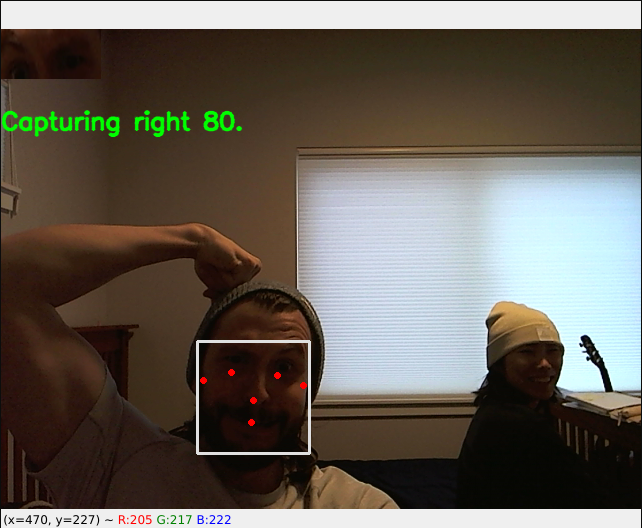
\includegraphics[width=0.9\columnwidth]{figures/Capturing-Example} 
	\caption{Example of the user interface during right raised eyebrow capture with only the closest face used.}
\end{figure}

\begin{figure}[ht!] % [h] forces the figure to be output where it is defined in the code (it suppresses floating)
	\centering
	\includegraphics[width=0.25\columnwidth]{../../../faceCNN/dataset/up/1000} 
	\includegraphics[width=0.25\columnwidth]{../../../faceCNN/dataset/down/1000} 
	\includegraphics[width=0.25\columnwidth]{../../../faceCNN/dataset/neutral/1000} 
	\includegraphics[width=0.25\columnwidth]{../../../faceCNN/dataset/left/1500} 
	\includegraphics[width=0.25\columnwidth]{../../../faceCNN/dataset/right/1000} 
	\caption{Example of images from the created dataset. Starting from top left: up, down, neutral,left, right.}
\end{figure}

\clearpage
\section{code}

All files related to this project can be found at: 

\url{https://github.com/Trenton-Ruf/Intelligent_Robotics}

\lstinputlisting[
	caption= faceCrop.py, % Caption above the listing
	%label=lst:test, % Label for referencing this listing
	language=Python, % Use Perl functions/syntax highlighting
	frame=single, % Frame around the code listing
	breaklines=true,
	postbreak=\mbox{\textcolor{red}{$\hookrightarrow$}\space},	
	showstringspaces=false, % Don't put marks in string spaces
	numbers=left, % Line numbers on left
	numberstyle=\tiny, % Line numbers styling
	basicstyle=\footnotesize
	]{../../../faceCNN/faceCrop.py}

\end{document}

